\documentclass[twoside]{book}

% Packages required by doxygen
\usepackage{fixltx2e}
\usepackage{calc}
\usepackage{doxygen}
\usepackage[export]{adjustbox} % also loads graphicx
\usepackage{graphicx}
\usepackage[utf8]{inputenc}
\usepackage{makeidx}
\usepackage{multicol}
\usepackage{multirow}
\PassOptionsToPackage{warn}{textcomp}
\usepackage{textcomp}
\usepackage[nointegrals]{wasysym}
\usepackage[table]{xcolor}

% Font selection
\usepackage[T1]{fontenc}
\usepackage[scaled=.90]{helvet}
\usepackage{courier}
\usepackage{amssymb}
\usepackage{sectsty}
\renewcommand{\familydefault}{\sfdefault}
\allsectionsfont{%
  \fontseries{bc}\selectfont%
  \color{darkgray}%
}
\renewcommand{\DoxyLabelFont}{%
  \fontseries{bc}\selectfont%
  \color{darkgray}%
}
\newcommand{\+}{\discretionary{\mbox{\scriptsize$\hookleftarrow$}}{}{}}

% Page & text layout
\usepackage{geometry}
\geometry{%
  a4paper,%
  top=2.5cm,%
  bottom=2.5cm,%
  left=2.5cm,%
  right=2.5cm%
}
\tolerance=750
\hfuzz=15pt
\hbadness=750
\setlength{\emergencystretch}{15pt}
\setlength{\parindent}{0cm}
\setlength{\parskip}{3ex plus 2ex minus 2ex}
\makeatletter
\renewcommand{\paragraph}{%
  \@startsection{paragraph}{4}{0ex}{-1.0ex}{1.0ex}{%
    \normalfont\normalsize\bfseries\SS@parafont%
  }%
}
\renewcommand{\subparagraph}{%
  \@startsection{subparagraph}{5}{0ex}{-1.0ex}{1.0ex}{%
    \normalfont\normalsize\bfseries\SS@subparafont%
  }%
}
\makeatother

% Headers & footers
\usepackage{fancyhdr}
\pagestyle{fancyplain}
\fancyhead[LE]{\fancyplain{}{\bfseries\thepage}}
\fancyhead[CE]{\fancyplain{}{}}
\fancyhead[RE]{\fancyplain{}{\bfseries\leftmark}}
\fancyhead[LO]{\fancyplain{}{\bfseries\rightmark}}
\fancyhead[CO]{\fancyplain{}{}}
\fancyhead[RO]{\fancyplain{}{\bfseries\thepage}}
\fancyfoot[LE]{\fancyplain{}{}}
\fancyfoot[CE]{\fancyplain{}{}}
\fancyfoot[RE]{\fancyplain{}{\bfseries\scriptsize Generated by Doxygen }}
\fancyfoot[LO]{\fancyplain{}{\bfseries\scriptsize Generated by Doxygen }}
\fancyfoot[CO]{\fancyplain{}{}}
\fancyfoot[RO]{\fancyplain{}{}}
\renewcommand{\footrulewidth}{0.4pt}
\renewcommand{\chaptermark}[1]{%
  \markboth{#1}{}%
}
\renewcommand{\sectionmark}[1]{%
  \markright{\thesection\ #1}%
}

% Indices & bibliography
\usepackage{natbib}
\usepackage[titles]{tocloft}
\setcounter{tocdepth}{3}
\setcounter{secnumdepth}{5}
\makeindex

% Hyperlinks (required, but should be loaded last)
\usepackage{ifpdf}
\ifpdf
  \usepackage[pdftex,pagebackref=true]{hyperref}
\else
  \usepackage[ps2pdf,pagebackref=true]{hyperref}
\fi
\hypersetup{%
  colorlinks=true,%
  linkcolor=blue,%
  citecolor=blue,%
  unicode%
}

% Custom commands
\newcommand{\clearemptydoublepage}{%
  \newpage{\pagestyle{empty}\cleardoublepage}%
}

\usepackage{caption}
\captionsetup{labelsep=space,justification=centering,font={bf},singlelinecheck=off,skip=4pt,position=top}

%===== C O N T E N T S =====

\begin{document}

% Titlepage & ToC
\hypersetup{pageanchor=false,
             bookmarksnumbered=true,
             pdfencoding=unicode
            }
\pagenumbering{alph}
\begin{titlepage}
\vspace*{7cm}
\begin{center}%
{\Large ip\+\_\+print }\\
\vspace*{1cm}
{\large Generated by Doxygen 1.8.13}\\
\end{center}
\end{titlepage}
\clearemptydoublepage
\pagenumbering{roman}
\tableofcontents
\clearemptydoublepage
\pagenumbering{arabic}
\hypersetup{pageanchor=true}

%--- Begin generated contents ---
\chapter{Hierarchical Index}
\section{Class Hierarchy}
This inheritance list is sorted roughly, but not completely, alphabetically\+:\begin{DoxyCompactList}
\item false\+\_\+type\begin{DoxyCompactList}
\item \contentsline{section}{is\+\_\+tuple$<$ T $>$}{\pageref{structis__tuple}}{}
\end{DoxyCompactList}
\item \contentsline{section}{has\+\_\+begin$<$ T $>$}{\pageref{structhas__begin}}{}
\item \contentsline{section}{has\+\_\+end$<$ T $>$}{\pageref{structhas__end}}{}
\item \contentsline{section}{is\+\_\+tuple\+\_\+integral$<$ T $>$}{\pageref{structis__tuple__integral}}{}
\item \contentsline{section}{is\+\_\+tuple\+\_\+same$<$ T $>$}{\pageref{structis__tuple__same}}{}
\end{DoxyCompactList}

\chapter{Class Index}
\section{Class List}
Here are the classes, structs, unions and interfaces with brief descriptions\+:\begin{DoxyCompactList}
\item\contentsline{section}{\hyperlink{structhas__begin}{has\+\_\+begin$<$ T $>$} \\*Check if type T has \textquotesingle{}begin()\textquotesingle{} method }{\pageref{structhas__begin}}{}
\item\contentsline{section}{\hyperlink{structhas__end}{has\+\_\+end$<$ T $>$} \\*Check if type T has \textquotesingle{}end()\textquotesingle{} method }{\pageref{structhas__end}}{}
\item\contentsline{section}{\hyperlink{structis__tuple}{is\+\_\+tuple$<$ T $>$} \\*Check if type T is tuple }{\pageref{structis__tuple}}{}
\item\contentsline{section}{\hyperlink{structis__tuple__integral}{is\+\_\+tuple\+\_\+integral$<$ T $>$} \\*Check if tuple T has all elements of the integral type }{\pageref{structis__tuple__integral}}{}
\item\contentsline{section}{\hyperlink{structis__tuple__same}{is\+\_\+tuple\+\_\+same$<$ T $>$} \\*Check if tuple T has all elements of the same type }{\pageref{structis__tuple__same}}{}
\end{DoxyCompactList}

\chapter{File Index}
\section{File List}
Here is a list of all files with brief descriptions\+:\begin{DoxyCompactList}
\item\contentsline{section}{src/\hyperlink{in_8version_8h}{in.\+version.\+h} }{\pageref{in_8version_8h}}{}
\item\contentsline{section}{src/\hyperlink{ip__print_8h}{ip\+\_\+print.\+h} }{\pageref{ip__print_8h}}{}
\item\contentsline{section}{src/\hyperlink{main_8cpp}{main.\+cpp} }{\pageref{main_8cpp}}{}
\item\contentsline{section}{src/\hyperlink{test_8cpp}{test.\+cpp} }{\pageref{test_8cpp}}{}
\end{DoxyCompactList}

\chapter{Class Documentation}
\hypertarget{structhas__begin}{}\section{has\+\_\+begin$<$ T $>$ Struct Template Reference}
\label{structhas__begin}\index{has\+\_\+begin$<$ T $>$@{has\+\_\+begin$<$ T $>$}}


check if type T has \textquotesingle{}begin()\textquotesingle{} method  




{\ttfamily \#include $<$ip\+\_\+print.\+h$>$}

\subsection*{Static Public Member Functions}
\begin{DoxyCompactItemize}
\item 
{\footnotesize template$<$typename U $>$ }\\static std\+::true\+\_\+type \hyperlink{structhas__begin_a9483204ce6d4d3de89ccd58f14e73cac}{test} (decltype(std\+::declval$<$ U $>$().begin()) $\ast$)
\item 
{\footnotesize template$<$typename U $>$ }\\static std\+::false\+\_\+type \hyperlink{structhas__begin_a47c984fb137d9cbe3db134c6a5a22550}{test} (...)
\end{DoxyCompactItemize}
\subsection*{Static Public Attributes}
\begin{DoxyCompactItemize}
\item 
static constexpr bool \hyperlink{structhas__begin_ae9ecdd6dfb43b08a7a028c5e8794359a}{value} = std\+::is\+\_\+same$<$ decltype(\hyperlink{structhas__begin_a9483204ce6d4d3de89ccd58f14e73cac}{test}$<$T$>$(nullptr)), std\+::true\+\_\+type$>$\+::value
\end{DoxyCompactItemize}


\subsection{Detailed Description}
\subsubsection*{template$<$typename T$>$\newline
struct has\+\_\+begin$<$ T $>$}

check if type T has \textquotesingle{}begin()\textquotesingle{} method 

\subsection{Member Function Documentation}
\mbox{\Hypertarget{structhas__begin_a9483204ce6d4d3de89ccd58f14e73cac}\label{structhas__begin_a9483204ce6d4d3de89ccd58f14e73cac}} 
\index{has\+\_\+begin@{has\+\_\+begin}!test@{test}}
\index{test@{test}!has\+\_\+begin@{has\+\_\+begin}}
\subsubsection{\texorpdfstring{test()}{test()}\hspace{0.1cm}{\footnotesize\ttfamily [1/2]}}
{\footnotesize\ttfamily template$<$typename T $>$ \\
template$<$typename U $>$ \\
static std\+::true\+\_\+type \hyperlink{structhas__begin}{has\+\_\+begin}$<$ T $>$\+::test (\begin{DoxyParamCaption}\item[{decltype(std\+::declval$<$ U $>$().begin()) $\ast$}]{ }\end{DoxyParamCaption})\hspace{0.3cm}{\ttfamily [static]}}

\mbox{\Hypertarget{structhas__begin_a47c984fb137d9cbe3db134c6a5a22550}\label{structhas__begin_a47c984fb137d9cbe3db134c6a5a22550}} 
\index{has\+\_\+begin@{has\+\_\+begin}!test@{test}}
\index{test@{test}!has\+\_\+begin@{has\+\_\+begin}}
\subsubsection{\texorpdfstring{test()}{test()}\hspace{0.1cm}{\footnotesize\ttfamily [2/2]}}
{\footnotesize\ttfamily template$<$typename T $>$ \\
template$<$typename U $>$ \\
static std\+::false\+\_\+type \hyperlink{structhas__begin}{has\+\_\+begin}$<$ T $>$\+::test (\begin{DoxyParamCaption}\item[{}]{... }\end{DoxyParamCaption})\hspace{0.3cm}{\ttfamily [static]}}



\subsection{Member Data Documentation}
\mbox{\Hypertarget{structhas__begin_ae9ecdd6dfb43b08a7a028c5e8794359a}\label{structhas__begin_ae9ecdd6dfb43b08a7a028c5e8794359a}} 
\index{has\+\_\+begin@{has\+\_\+begin}!value@{value}}
\index{value@{value}!has\+\_\+begin@{has\+\_\+begin}}
\subsubsection{\texorpdfstring{value}{value}}
{\footnotesize\ttfamily template$<$typename T $>$ \\
constexpr bool \hyperlink{structhas__begin}{has\+\_\+begin}$<$ T $>$\+::value = std\+::is\+\_\+same$<$ decltype(\hyperlink{structhas__begin_a9483204ce6d4d3de89ccd58f14e73cac}{test}$<$T$>$(nullptr)), std\+::true\+\_\+type$>$\+::value\hspace{0.3cm}{\ttfamily [static]}}



The documentation for this struct was generated from the following file\+:\begin{DoxyCompactItemize}
\item 
src/\hyperlink{ip__print_8h}{ip\+\_\+print.\+h}\end{DoxyCompactItemize}

\hypertarget{structhas__end}{}\section{has\+\_\+end$<$ T $>$ Struct Template Reference}
\label{structhas__end}\index{has\+\_\+end$<$ T $>$@{has\+\_\+end$<$ T $>$}}


check if type T has \textquotesingle{}end()\textquotesingle{} method  




{\ttfamily \#include $<$ip\+\_\+print.\+h$>$}

\subsection*{Static Public Member Functions}
\begin{DoxyCompactItemize}
\item 
{\footnotesize template$<$typename U $>$ }\\static std\+::true\+\_\+type \hyperlink{structhas__end_aa7f205d85237693f6d331008ca208caa}{test} (decltype(std\+::declval$<$ U $>$().end()) $\ast$)
\item 
{\footnotesize template$<$typename U $>$ }\\static std\+::false\+\_\+type \hyperlink{structhas__end_a7271796b8a3415685dd533aee13f9619}{test} (...)
\end{DoxyCompactItemize}
\subsection*{Static Public Attributes}
\begin{DoxyCompactItemize}
\item 
static constexpr bool \hyperlink{structhas__end_ae73ed670937d854009087106a4c181a4}{value} = std\+::is\+\_\+same$<$ decltype(\hyperlink{structhas__end_aa7f205d85237693f6d331008ca208caa}{test}$<$T$>$(nullptr)), std\+::true\+\_\+type$>$\+::value
\end{DoxyCompactItemize}


\subsection{Detailed Description}
\subsubsection*{template$<$typename T$>$\newline
struct has\+\_\+end$<$ T $>$}

check if type T has \textquotesingle{}end()\textquotesingle{} method 

\subsection{Member Function Documentation}
\mbox{\Hypertarget{structhas__end_aa7f205d85237693f6d331008ca208caa}\label{structhas__end_aa7f205d85237693f6d331008ca208caa}} 
\index{has\+\_\+end@{has\+\_\+end}!test@{test}}
\index{test@{test}!has\+\_\+end@{has\+\_\+end}}
\subsubsection{\texorpdfstring{test()}{test()}\hspace{0.1cm}{\footnotesize\ttfamily [1/2]}}
{\footnotesize\ttfamily template$<$typename T $>$ \\
template$<$typename U $>$ \\
static std\+::true\+\_\+type \hyperlink{structhas__end}{has\+\_\+end}$<$ T $>$\+::test (\begin{DoxyParamCaption}\item[{decltype(std\+::declval$<$ U $>$().end()) $\ast$}]{ }\end{DoxyParamCaption})\hspace{0.3cm}{\ttfamily [static]}}

\mbox{\Hypertarget{structhas__end_a7271796b8a3415685dd533aee13f9619}\label{structhas__end_a7271796b8a3415685dd533aee13f9619}} 
\index{has\+\_\+end@{has\+\_\+end}!test@{test}}
\index{test@{test}!has\+\_\+end@{has\+\_\+end}}
\subsubsection{\texorpdfstring{test()}{test()}\hspace{0.1cm}{\footnotesize\ttfamily [2/2]}}
{\footnotesize\ttfamily template$<$typename T $>$ \\
template$<$typename U $>$ \\
static std\+::false\+\_\+type \hyperlink{structhas__end}{has\+\_\+end}$<$ T $>$\+::test (\begin{DoxyParamCaption}\item[{}]{... }\end{DoxyParamCaption})\hspace{0.3cm}{\ttfamily [static]}}



\subsection{Member Data Documentation}
\mbox{\Hypertarget{structhas__end_ae73ed670937d854009087106a4c181a4}\label{structhas__end_ae73ed670937d854009087106a4c181a4}} 
\index{has\+\_\+end@{has\+\_\+end}!value@{value}}
\index{value@{value}!has\+\_\+end@{has\+\_\+end}}
\subsubsection{\texorpdfstring{value}{value}}
{\footnotesize\ttfamily template$<$typename T $>$ \\
constexpr bool \hyperlink{structhas__end}{has\+\_\+end}$<$ T $>$\+::value = std\+::is\+\_\+same$<$ decltype(\hyperlink{structhas__end_aa7f205d85237693f6d331008ca208caa}{test}$<$T$>$(nullptr)), std\+::true\+\_\+type$>$\+::value\hspace{0.3cm}{\ttfamily [static]}}



The documentation for this struct was generated from the following file\+:\begin{DoxyCompactItemize}
\item 
src/\hyperlink{ip__print_8h}{ip\+\_\+print.\+h}\end{DoxyCompactItemize}

\hypertarget{structis__tuple}{}\section{is\+\_\+tuple$<$ T $>$ Struct Template Reference}
\label{structis__tuple}\index{is\+\_\+tuple$<$ T $>$@{is\+\_\+tuple$<$ T $>$}}


check if type T is tuple  




{\ttfamily \#include $<$ip\+\_\+print.\+h$>$}



Inheritance diagram for is\+\_\+tuple$<$ T $>$\+:
\nopagebreak
\begin{figure}[H]
\begin{center}
\leavevmode
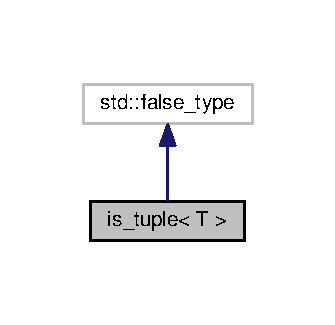
\includegraphics[width=161pt]{structis__tuple__inherit__graph}
\end{center}
\end{figure}


Collaboration diagram for is\+\_\+tuple$<$ T $>$\+:
\nopagebreak
\begin{figure}[H]
\begin{center}
\leavevmode
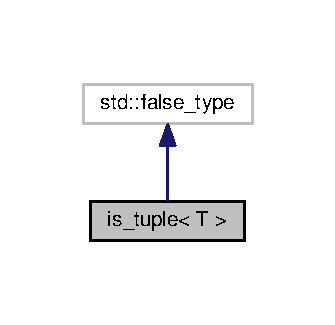
\includegraphics[width=161pt]{structis__tuple__coll__graph}
\end{center}
\end{figure}


\subsection{Detailed Description}
\subsubsection*{template$<$typename T$>$\newline
struct is\+\_\+tuple$<$ T $>$}

check if type T is tuple 

The documentation for this struct was generated from the following file\+:\begin{DoxyCompactItemize}
\item 
src/\hyperlink{ip__print_8h}{ip\+\_\+print.\+h}\end{DoxyCompactItemize}

\hypertarget{structis__tuple__integral}{}\section{is\+\_\+tuple\+\_\+integral$<$ T $>$ Struct Template Reference}
\label{structis__tuple__integral}\index{is\+\_\+tuple\+\_\+integral$<$ T $>$@{is\+\_\+tuple\+\_\+integral$<$ T $>$}}


check if tuple T has all elements of the integral type  




{\ttfamily \#include $<$ip\+\_\+print.\+h$>$}



\subsection{Detailed Description}
\subsubsection*{template$<$typename T$>$\newline
struct is\+\_\+tuple\+\_\+integral$<$ T $>$}

check if tuple T has all elements of the integral type 

The documentation for this struct was generated from the following file\+:\begin{DoxyCompactItemize}
\item 
src/\hyperlink{ip__print_8h}{ip\+\_\+print.\+h}\end{DoxyCompactItemize}

\hypertarget{structis__tuple__same}{}\section{is\+\_\+tuple\+\_\+same$<$ T $>$ Struct Template Reference}
\label{structis__tuple__same}\index{is\+\_\+tuple\+\_\+same$<$ T $>$@{is\+\_\+tuple\+\_\+same$<$ T $>$}}


check if tuple T has all elements of the same type  




{\ttfamily \#include $<$ip\+\_\+print.\+h$>$}



\subsection{Detailed Description}
\subsubsection*{template$<$typename T$>$\newline
struct is\+\_\+tuple\+\_\+same$<$ T $>$}

check if tuple T has all elements of the same type 

The documentation for this struct was generated from the following file\+:\begin{DoxyCompactItemize}
\item 
src/\hyperlink{ip__print_8h}{ip\+\_\+print.\+h}\end{DoxyCompactItemize}

\chapter{File Documentation}
\hypertarget{in_8version_8h}{}\section{src/in.version.\+h File Reference}
\label{in_8version_8h}\index{src/in.\+version.\+h@{src/in.\+version.\+h}}
\subsection*{Macros}
\begin{DoxyCompactItemize}
\item 
\#define \hyperlink{in_8version_8h_a4a5fc96a4bdd7d68ed99ccce9ca2e77e}{P\+R\+O\+J\+E\+C\+T\+\_\+\+V\+E\+R\+S\+I\+O\+N\+\_\+\+P\+A\+T\+CH}~@P\+R\+O\+J\+E\+C\+T\+\_\+\+V\+E\+R\+S\+I\+O\+N\+\_\+\+P\+A\+T\+CH@
\end{DoxyCompactItemize}
\subsection*{Functions}
\begin{DoxyCompactItemize}
\item 
int \hyperlink{in_8version_8h_a4eef9c27a3287b7cfaa3c5374873b7be}{build\+\_\+version} ()
\end{DoxyCompactItemize}


\subsection{Macro Definition Documentation}
\mbox{\Hypertarget{in_8version_8h_a4a5fc96a4bdd7d68ed99ccce9ca2e77e}\label{in_8version_8h_a4a5fc96a4bdd7d68ed99ccce9ca2e77e}} 
\index{in.\+version.\+h@{in.\+version.\+h}!P\+R\+O\+J\+E\+C\+T\+\_\+\+V\+E\+R\+S\+I\+O\+N\+\_\+\+P\+A\+T\+CH@{P\+R\+O\+J\+E\+C\+T\+\_\+\+V\+E\+R\+S\+I\+O\+N\+\_\+\+P\+A\+T\+CH}}
\index{P\+R\+O\+J\+E\+C\+T\+\_\+\+V\+E\+R\+S\+I\+O\+N\+\_\+\+P\+A\+T\+CH@{P\+R\+O\+J\+E\+C\+T\+\_\+\+V\+E\+R\+S\+I\+O\+N\+\_\+\+P\+A\+T\+CH}!in.\+version.\+h@{in.\+version.\+h}}
\subsubsection{\texorpdfstring{P\+R\+O\+J\+E\+C\+T\+\_\+\+V\+E\+R\+S\+I\+O\+N\+\_\+\+P\+A\+T\+CH}{PROJECT\_VERSION\_PATCH}}
{\footnotesize\ttfamily \#define P\+R\+O\+J\+E\+C\+T\+\_\+\+V\+E\+R\+S\+I\+O\+N\+\_\+\+P\+A\+T\+CH~@P\+R\+O\+J\+E\+C\+T\+\_\+\+V\+E\+R\+S\+I\+O\+N\+\_\+\+P\+A\+T\+CH@}



\subsection{Function Documentation}
\mbox{\Hypertarget{in_8version_8h_a4eef9c27a3287b7cfaa3c5374873b7be}\label{in_8version_8h_a4eef9c27a3287b7cfaa3c5374873b7be}} 
\index{in.\+version.\+h@{in.\+version.\+h}!build\+\_\+version@{build\+\_\+version}}
\index{build\+\_\+version@{build\+\_\+version}!in.\+version.\+h@{in.\+version.\+h}}
\subsubsection{\texorpdfstring{build\+\_\+version()}{build\_version()}}
{\footnotesize\ttfamily int build\+\_\+version (\begin{DoxyParamCaption}{ }\end{DoxyParamCaption})\hspace{0.3cm}{\ttfamily [inline]}}


\hypertarget{ip__print_8h}{}\section{src/ip\+\_\+print.h File Reference}
\label{ip__print_8h}\index{src/ip\+\_\+print.\+h@{src/ip\+\_\+print.\+h}}
{\ttfamily \#include $<$iostream$>$}\newline
{\ttfamily \#include $<$type\+\_\+traits$>$}\newline
Include dependency graph for ip\+\_\+print.\+h\+:
\nopagebreak
\begin{figure}[H]
\begin{center}
\leavevmode
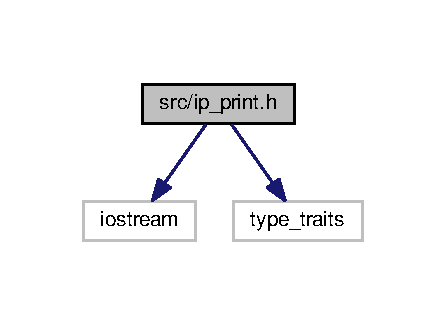
\includegraphics[width=214pt]{ip__print_8h__incl}
\end{center}
\end{figure}
This graph shows which files directly or indirectly include this file\+:
\nopagebreak
\begin{figure}[H]
\begin{center}
\leavevmode
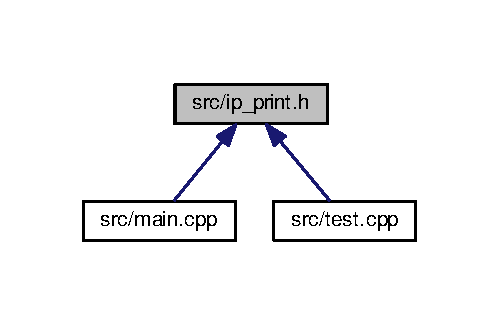
\includegraphics[width=240pt]{ip__print_8h__dep__incl}
\end{center}
\end{figure}
\subsection*{Classes}
\begin{DoxyCompactItemize}
\item 
struct \hyperlink{structhas__begin}{has\+\_\+begin$<$ T $>$}
\begin{DoxyCompactList}\small\item\em check if type T has \textquotesingle{}begin()\textquotesingle{} method \end{DoxyCompactList}\item 
struct \hyperlink{structhas__end}{has\+\_\+end$<$ T $>$}
\begin{DoxyCompactList}\small\item\em check if type T has \textquotesingle{}end()\textquotesingle{} method \end{DoxyCompactList}\item 
struct \hyperlink{structis__tuple}{is\+\_\+tuple$<$ T $>$}
\begin{DoxyCompactList}\small\item\em check if type T is tuple \end{DoxyCompactList}\item 
struct \hyperlink{structis__tuple__same}{is\+\_\+tuple\+\_\+same$<$ T $>$}
\begin{DoxyCompactList}\small\item\em check if tuple T has all elements of the same type \end{DoxyCompactList}\item 
struct \hyperlink{structis__tuple__integral}{is\+\_\+tuple\+\_\+integral$<$ T $>$}
\begin{DoxyCompactList}\small\item\em check if tuple T has all elements of the integral type \end{DoxyCompactList}\end{DoxyCompactItemize}
\subsection*{Functions}
\begin{DoxyCompactItemize}
\item 
{\footnotesize template$<$class T $>$ }\\std\+::string \hyperlink{ip__print_8h_a9f3a0223dc52c156a797906ecf696562}{pretty\+\_\+type\+\_\+name} ()
\begin{DoxyCompactList}\small\item\em function provided for type of T to be printed \end{DoxyCompactList}\item 
{\footnotesize template$<$typename T $>$ }\\std\+::ostream \& \hyperlink{ip__print_8h_ae241e51a484f0430540953e328da150f}{ip\+\_\+print} (const T \&t, std\+::ostream \&os)
\begin{DoxyCompactList}\small\item\em ip print from varuous types \end{DoxyCompactList}\end{DoxyCompactItemize}
\textbf{ }\par



\subsection{Detailed Description}
ip\+\_\+print implementation 

\subsection{Function Documentation}
\mbox{\Hypertarget{ip__print_8h_ae241e51a484f0430540953e328da150f}\label{ip__print_8h_ae241e51a484f0430540953e328da150f}} 
\index{ip\+\_\+print.\+h@{ip\+\_\+print.\+h}!ip\+\_\+print@{ip\+\_\+print}}
\index{ip\+\_\+print@{ip\+\_\+print}!ip\+\_\+print.\+h@{ip\+\_\+print.\+h}}
\subsubsection{\texorpdfstring{ip\+\_\+print()}{ip\_print()}}
{\footnotesize\ttfamily template$<$typename T $>$ \\
std\+::ostream\& ip\+\_\+print (\begin{DoxyParamCaption}\item[{const T \&}]{t,  }\item[{std\+::ostream \&}]{os }\end{DoxyParamCaption})}



ip print from varuous types 

\mbox{\Hypertarget{ip__print_8h_a9f3a0223dc52c156a797906ecf696562}\label{ip__print_8h_a9f3a0223dc52c156a797906ecf696562}} 
\index{ip\+\_\+print.\+h@{ip\+\_\+print.\+h}!pretty\+\_\+type\+\_\+name@{pretty\+\_\+type\+\_\+name}}
\index{pretty\+\_\+type\+\_\+name@{pretty\+\_\+type\+\_\+name}!ip\+\_\+print.\+h@{ip\+\_\+print.\+h}}
\subsubsection{\texorpdfstring{pretty\+\_\+type\+\_\+name()}{pretty\_type\_name()}}
{\footnotesize\ttfamily template$<$class T $>$ \\
std\+::string pretty\+\_\+type\+\_\+name (\begin{DoxyParamCaption}{ }\end{DoxyParamCaption})}



function provided for type of T to be printed 


\hypertarget{main_8cpp}{}\section{src/main.cpp File Reference}
\label{main_8cpp}\index{src/main.\+cpp@{src/main.\+cpp}}
{\ttfamily \#include $<$iostream$>$}\newline
{\ttfamily \#include $<$boost/program\+\_\+options.\+hpp$>$}\newline
{\ttfamily \#include \char`\"{}../bin/version.\+h\char`\"{}}\newline
{\ttfamily \#include $<$vector$>$}\newline
{\ttfamily \#include $<$list$>$}\newline
{\ttfamily \#include $<$tuple$>$}\newline
{\ttfamily \#include \char`\"{}ip\+\_\+print.\+h\char`\"{}}\newline
Include dependency graph for main.\+cpp\+:
\nopagebreak
\begin{figure}[H]
\begin{center}
\leavevmode
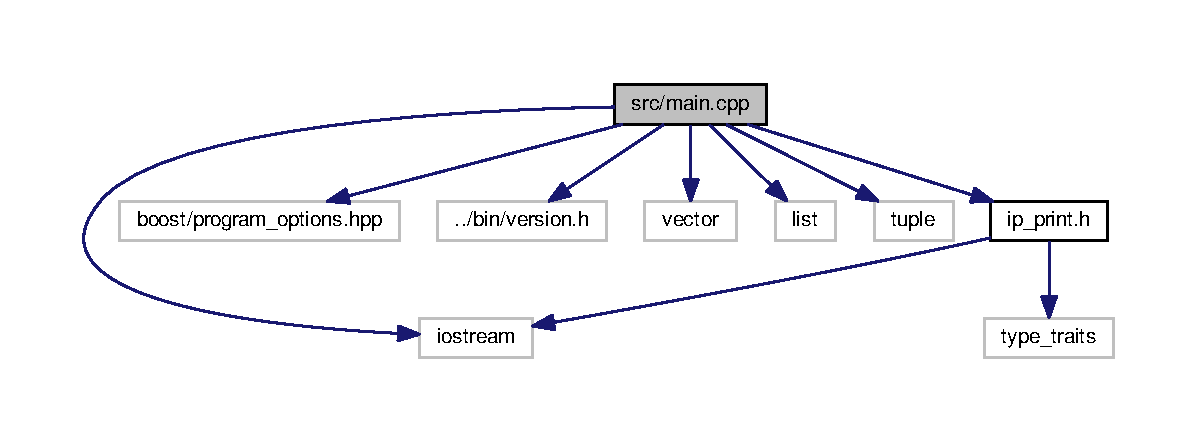
\includegraphics[width=350pt]{main_8cpp__incl}
\end{center}
\end{figure}
\subsection*{Functions}
\begin{DoxyCompactItemize}
\item 
int \hyperlink{main_8cpp_a3c04138a5bfe5d72780bb7e82a18e627}{main} (int argc, char $\ast$$\ast$argv)
\end{DoxyCompactItemize}


\subsection{Detailed Description}
application entry point

Usage\+:

-\/-\/help,-\/h print help

-\/-\/version,-\/v print application and boost version 

\subsection{Function Documentation}
\mbox{\Hypertarget{main_8cpp_a3c04138a5bfe5d72780bb7e82a18e627}\label{main_8cpp_a3c04138a5bfe5d72780bb7e82a18e627}} 
\index{main.\+cpp@{main.\+cpp}!main@{main}}
\index{main@{main}!main.\+cpp@{main.\+cpp}}
\subsubsection{\texorpdfstring{main()}{main()}}
{\footnotesize\ttfamily int main (\begin{DoxyParamCaption}\item[{int}]{argc,  }\item[{char $\ast$$\ast$}]{argv }\end{DoxyParamCaption})}


\hypertarget{test_8cpp}{}\section{src/test.cpp File Reference}
\label{test_8cpp}\index{src/test.\+cpp@{src/test.\+cpp}}
{\ttfamily \#include $<$boost/test/unit\+\_\+test.\+hpp$>$}\newline
{\ttfamily \#include $<$sstream$>$}\newline
{\ttfamily \#include $<$vector$>$}\newline
{\ttfamily \#include $<$list$>$}\newline
{\ttfamily \#include $<$deque$>$}\newline
{\ttfamily \#include \char`\"{}../bin/version.\+h\char`\"{}}\newline
{\ttfamily \#include \char`\"{}ip\+\_\+print.\+h\char`\"{}}\newline
Include dependency graph for test.\+cpp\+:
\nopagebreak
\begin{figure}[H]
\begin{center}
\leavevmode
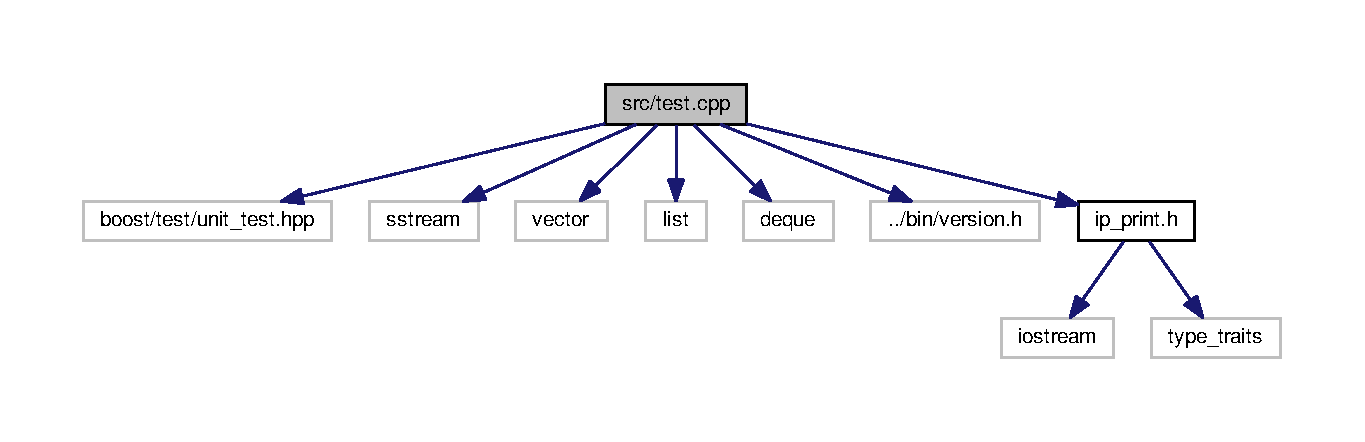
\includegraphics[width=350pt]{test_8cpp__incl}
\end{center}
\end{figure}
\subsection*{Macros}
\begin{DoxyCompactItemize}
\item 
\#define \hyperlink{test_8cpp_a6b2a3852db8bb19ab6909bac01859985}{B\+O\+O\+S\+T\+\_\+\+T\+E\+S\+T\+\_\+\+M\+O\+D\+U\+LE}~Test\+Main
\end{DoxyCompactItemize}
\subsection*{Functions}
\begin{DoxyCompactItemize}
\item 
{\footnotesize template$<$typename T $>$ }\\std\+::string \hyperlink{test_8cpp_a4b33397cd5a5a28b9c388d1b1342400c}{ip2str} (const T \&t)
\begin{DoxyCompactList}\small\item\em test helper, print ip from class T to string \end{DoxyCompactList}\item 
{\footnotesize template$<$typename T $>$ }\\void \hyperlink{test_8cpp_ace347b84b3954f7ddcac24b6138aa188}{test\+\_\+array} ()
\begin{DoxyCompactList}\small\item\em test helper, make tests to print ip from array of T \end{DoxyCompactList}\item 
{\footnotesize template$<$typename T $>$ }\\void \hyperlink{test_8cpp_ad540da47ecb368efa940524e7e6186a3}{test\+\_\+container} ()
\begin{DoxyCompactList}\small\item\em test helper, make tests to print ip from container T \end{DoxyCompactList}\item 
{\footnotesize template$<$typename T $>$ }\\void \hyperlink{test_8cpp_aa150aab97d9d80fbf3f11a1730a62fe6}{test\+\_\+container\+\_\+negative} ()
\begin{DoxyCompactList}\small\item\em test helper, make tests to print ip from containers of T which have negative octets \end{DoxyCompactList}\item 
{\footnotesize template$<$typename T $>$ }\\void \hyperlink{test_8cpp_ae93d9fa7248444377f35f85603c13f0f}{test\+\_\+tuple} ()
\begin{DoxyCompactList}\small\item\em test helper, make tests to print ip from tuple of T \end{DoxyCompactList}\end{DoxyCompactItemize}


\subsection{Detailed Description}
ip\+\_\+print testing 

\subsection{Macro Definition Documentation}
\mbox{\Hypertarget{test_8cpp_a6b2a3852db8bb19ab6909bac01859985}\label{test_8cpp_a6b2a3852db8bb19ab6909bac01859985}} 
\index{test.\+cpp@{test.\+cpp}!B\+O\+O\+S\+T\+\_\+\+T\+E\+S\+T\+\_\+\+M\+O\+D\+U\+LE@{B\+O\+O\+S\+T\+\_\+\+T\+E\+S\+T\+\_\+\+M\+O\+D\+U\+LE}}
\index{B\+O\+O\+S\+T\+\_\+\+T\+E\+S\+T\+\_\+\+M\+O\+D\+U\+LE@{B\+O\+O\+S\+T\+\_\+\+T\+E\+S\+T\+\_\+\+M\+O\+D\+U\+LE}!test.\+cpp@{test.\+cpp}}
\subsubsection{\texorpdfstring{B\+O\+O\+S\+T\+\_\+\+T\+E\+S\+T\+\_\+\+M\+O\+D\+U\+LE}{BOOST\_TEST\_MODULE}}
{\footnotesize\ttfamily \#define B\+O\+O\+S\+T\+\_\+\+T\+E\+S\+T\+\_\+\+M\+O\+D\+U\+LE~Test\+Main}



\subsection{Function Documentation}
\mbox{\Hypertarget{test_8cpp_a4b33397cd5a5a28b9c388d1b1342400c}\label{test_8cpp_a4b33397cd5a5a28b9c388d1b1342400c}} 
\index{test.\+cpp@{test.\+cpp}!ip2str@{ip2str}}
\index{ip2str@{ip2str}!test.\+cpp@{test.\+cpp}}
\subsubsection{\texorpdfstring{ip2str()}{ip2str()}}
{\footnotesize\ttfamily template$<$typename T $>$ \\
std\+::string ip2str (\begin{DoxyParamCaption}\item[{const T \&}]{t }\end{DoxyParamCaption})}



test helper, print ip from class T to string 

\mbox{\Hypertarget{test_8cpp_ace347b84b3954f7ddcac24b6138aa188}\label{test_8cpp_ace347b84b3954f7ddcac24b6138aa188}} 
\index{test.\+cpp@{test.\+cpp}!test\+\_\+array@{test\+\_\+array}}
\index{test\+\_\+array@{test\+\_\+array}!test.\+cpp@{test.\+cpp}}
\subsubsection{\texorpdfstring{test\+\_\+array()}{test\_array()}}
{\footnotesize\ttfamily template$<$typename T $>$ \\
void test\+\_\+array (\begin{DoxyParamCaption}{ }\end{DoxyParamCaption})}



test helper, make tests to print ip from array of T 

\mbox{\Hypertarget{test_8cpp_ad540da47ecb368efa940524e7e6186a3}\label{test_8cpp_ad540da47ecb368efa940524e7e6186a3}} 
\index{test.\+cpp@{test.\+cpp}!test\+\_\+container@{test\+\_\+container}}
\index{test\+\_\+container@{test\+\_\+container}!test.\+cpp@{test.\+cpp}}
\subsubsection{\texorpdfstring{test\+\_\+container()}{test\_container()}}
{\footnotesize\ttfamily template$<$typename T $>$ \\
void test\+\_\+container (\begin{DoxyParamCaption}{ }\end{DoxyParamCaption})}



test helper, make tests to print ip from container T 

\mbox{\Hypertarget{test_8cpp_aa150aab97d9d80fbf3f11a1730a62fe6}\label{test_8cpp_aa150aab97d9d80fbf3f11a1730a62fe6}} 
\index{test.\+cpp@{test.\+cpp}!test\+\_\+container\+\_\+negative@{test\+\_\+container\+\_\+negative}}
\index{test\+\_\+container\+\_\+negative@{test\+\_\+container\+\_\+negative}!test.\+cpp@{test.\+cpp}}
\subsubsection{\texorpdfstring{test\+\_\+container\+\_\+negative()}{test\_container\_negative()}}
{\footnotesize\ttfamily template$<$typename T $>$ \\
void test\+\_\+container\+\_\+negative (\begin{DoxyParamCaption}{ }\end{DoxyParamCaption})}



test helper, make tests to print ip from containers of T which have negative octets 

\mbox{\Hypertarget{test_8cpp_ae93d9fa7248444377f35f85603c13f0f}\label{test_8cpp_ae93d9fa7248444377f35f85603c13f0f}} 
\index{test.\+cpp@{test.\+cpp}!test\+\_\+tuple@{test\+\_\+tuple}}
\index{test\+\_\+tuple@{test\+\_\+tuple}!test.\+cpp@{test.\+cpp}}
\subsubsection{\texorpdfstring{test\+\_\+tuple()}{test\_tuple()}}
{\footnotesize\ttfamily template$<$typename T $>$ \\
void test\+\_\+tuple (\begin{DoxyParamCaption}{ }\end{DoxyParamCaption})}



test helper, make tests to print ip from tuple of T 


%--- End generated contents ---

% Index
\backmatter
\newpage
\phantomsection
\clearemptydoublepage
\addcontentsline{toc}{chapter}{Index}
\printindex

\end{document}
